% INT4096 group presentation — restructured as a five-act research story.
% Build: bash slides/build.sh
%
% Speaker roles below are PRESENTATION roles only. They are not statements about
% who did the software, the experiments or the research: see
% docs/management/responsibilities.md for actual ownership.
%
% Every empirical number is a macro from generated/numbers.tex, produced from
% artifacts/experiments by scripts/build_slide_assets.py. Nothing is typed by hand.
\documentclass[aspectratio=169,11pt]{beamer}

\usetheme{metropolis}
\usepackage[T1]{fontenc}
\usepackage{lmodern}
\usepackage{booktabs}
\usepackage{graphicx}
\usepackage{siunitx}
\usepackage{tikz}
\usetikzlibrary{arrows.meta,positioning}

\sisetup{detect-all}
% beamer's \appendix writes \translate into a PDF bookmark; hyperref cannot put
% it in a string and warns. This is the documented remedy.
\pdfstringdefDisableCommands{\def\translate#1{}}
\hypersetup{pdftitle={Can Five Machine-Learning Models Beat a One-Line Rule?},
            pdfsubject={INT4096 group project presentation},
            pdfkeywords={machine learning, time series, baselines, leakage}}
\graphicspath{{figures/}}
% GENERATED by scripts/build_slide_assets.py -- do not edit by hand.
% Sources: artifacts/experiments/*/{manifest,metrics,config,predictions}
%          artifacts/analysis/uncertainty_and_signal.json
\newcommand{\NRunTotal}{20}
\newcommand{\NPairTotal}{10}
\newcommand{\NBelowBaseline}{5}
\newcommand{\NPairsBelowBaseline}{3}
\newcommand{\BestAAPLModelAll}{SVR (RBF)}
\newcommand{\BestAAPLVariantAll}{P2}
\newcommand{\BestAAPLSkillAll}{+0.52}
\newcommand{\BestAAPLModelPtwo}{SVR (RBF)}
\newcommand{\BestAAPLSkillPtwo}{+0.52}
\newcommand{\NaiveMaeAAPL}{2.91}
\newcommand{\NValObsAAPL}{244}
\newcommand{\SkillAAPLLinearBaseline}{-0.50}
\newcommand{\MaeAAPLLinearBaseline}{2.92}
\newcommand{\SkillAAPLRidge}{+0.29}
\newcommand{\MaeAAPLRidge}{2.90}
\newcommand{\SkillAAPLSvr}{+0.52}
\newcommand{\MaeAAPLSvr}{2.89}
\newcommand{\SkillAAPLRandomForest}{-0.78}
\newcommand{\MaeAAPLRandomForest}{2.93}
\newcommand{\SkillAAPLHistGradientBoosting}{+0.25}
\newcommand{\MaeAAPLHistGradientBoosting}{2.90}
\newcommand{\BestBTCModelAll}{Linear baseline}
\newcommand{\BestBTCVariantAll}{P0}
\newcommand{\BestBTCSkillAll}{+0.26}
\newcommand{\BestBTCModelPtwo}{Ridge}
\newcommand{\BestBTCSkillPtwo}{+0.12}
\newcommand{\NaiveMaeBTC}{1604.35}
\newcommand{\NValObsBTC}{358}
\newcommand{\SkillBTCLinearBaseline}{+0.05}
\newcommand{\MaeBTCLinearBaseline}{1603.59}
\newcommand{\SkillBTCRidge}{+0.12}
\newcommand{\MaeBTCRidge}{1602.39}
\newcommand{\SkillBTCSvr}{+0.08}
\newcommand{\MaeBTCSvr}{1603.13}
\newcommand{\SkillBTCRandomForest}{+0.06}
\newcommand{\MaeBTCRandomForest}{1603.37}
\newcommand{\SkillBTCHistGradientBoosting}{-0.04}
\newcommand{\MaeBTCHistGradientBoosting}{1605.02}
\newcommand{\SkillMin}{-0.78}
\newcommand{\SkillMax}{+0.52}
\newcommand{\SkillSpan}{1.30}
\newcommand{\TrialsUsed}{10}
\newcommand{\SecondsUsed}{90}
\newcommand{\TrialsMax}{24}
\newcommand{\SecondsMax}{300}
\newcommand{\BudgetUniform}{yes}
\newcommand{\AnalysisPresent}{yes}
\newcommand{\AutoAAPL}{+0.021}
\newcommand{\AutoRsqAAPL}{0.0005}
\newcommand{\AutoBTC}{-0.026}
\newcommand{\AutoRsqBTC}{0.0007}
\newcommand{\NCiTotal}{20}
\newcommand{\NCiIncludeZero}{20}
\newcommand{\CiBlock}{10}
\newcommand{\CiResamples}{1{,}000}
\newcommand{\ExDate}{2024-11-21}
\newcommand{\ExCt}{228.52}
\newcommand{\ExDelta}{+0.10}
\newcommand{\ExPred}{228.62}
\newcommand{\ExActual}{229.87}
\newcommand{\ExErr}{1.25}
\newcommand{\ExNaiveErr}{1.35}
\newcommand{\TreeMeasured}{yes}
\newcommand{\TreeMaxDiff}{0}
\newcommand{\TreeExact}{zero}
\newcommand{\TreeVerdict}{exactly zero}
\newcommand{\NumPtwoRuns}{10}
\newcommand{\NumPtwoNegative}{3}
\newcommand{\NumAllNegative}{5}
\newcommand{\LinAAPLPzeroMae}{2.90}
\newcommand{\LinAAPLPtwoMae}{2.92}
\newcommand{\LinAAPLDeltaPct}{+0.74}
\newcommand{\BestBTCOverallSkill}{+0.26}
\newcommand{\BestBTCOverallConfig}{Linear baseline, P0}
\newcommand{\ObsAAPL}{1{,}255}
\newcommand{\ObsBTC}{1{,}828}
\newcommand{\NMutations}{6}
\newcommand{\LeakDelta}{0.408}
\newcommand{\HookAAPLRsq}{0.9556}
\newcommand{\HookAAPLPersistenceRsq}{0.9555}
\newcommand{\AAPLGainCents}{1.5}
\newcommand{\WindowAAPL}{2021-10-28--2026-10-28}
\newcommand{\CloseRangeAAPL}{125--348}
\newcommand{\QualityAAPL}{PASS}
\newcommand{\WindowBTC}{2021-10-28--2026-10-29}
\newcommand{\CloseRangeBTC}{15{,}781--124{,}659}
\newcommand{\QualityBTC}{PASS}
\newcommand{\TrainAAPL}{2021-12-10--2024-11-08}
\newcommand{\ValAAPL}{2024-11-12--2025-11-03}
\newcommand{\TestAAPL}{2025-11-05--2026-10-27}
\newcommand{\NBarsAAPL}{1{,}255}
\newcommand{\TrainBTC}{2021-11-27--2024-11-07}
\newcommand{\ValBTC}{2024-11-09--2025-11-01}
\newcommand{\TestBTC}{2025-11-03--2026-10-28}
\newcommand{\NBarsBTC}{1{,}828}


\metroset{block=fill, sectionpage=none, numbering=fraction}
\setbeamercolor{author in head/foot}{bg=black!82,fg=white}
\setbeamercolor{date in head/foot}{bg=black!82,fg=white}

% Speaker attribution sits in the footer and is set from inside each frame.
\newcommand{\currentspeaker}{}
\newcommand{\speaker}[1]{\gdef\currentspeaker{#1}}

\newcommand{\intfootline}{%
  \leavevmode%
  \hbox{%
    \begin{beamercolorbox}[wd=.70\paperwidth,ht=2.4ex,dp=1.1ex,leftskip=.3cm]{author in head/foot}%
      \usebeamerfont{author in head/foot}\insertsectionhead\ ---\ \currentspeaker
    \end{beamercolorbox}%
    \begin{beamercolorbox}[wd=.30\paperwidth,ht=2.4ex,dp=1.1ex,right,rightskip=.3cm]{date in head/foot}%
      \usebeamerfont{date in head/foot}\insertframenumber\,/\,\inserttotalframenumber
    \end{beamercolorbox}%
  }\vskip0pt%
}
\setbeamertemplate{footline}{\intfootline}

\setbeamerfont{author}{size=\small}
\setbeamerfont{institute}{size=\scriptsize}

\title{Can Five Machine-Learning Models Beat a One-Line Rule?}
\subtitle{AAPL and BTC, one fair protocol, and what the answer teaches}
\author[INT4096]{%
  Zhang Yancheng \and Dong Yuankun \and Zhang Haoyu \and Lau Pak Hei \and Lui Shing Lam}
\institute{INT4096 AI and Machine Learning in Education\\
  The Education University of Hong Kong, Semester 1, 2026--27}
\date{}

\newcommand{\act}[1]{\section{#1}}

\begin{document}

% ===================================================== ACT I — THE CHALLENGE
% Lau Pak Hei, 1:20
\begin{frame}
  \speaker{Lau Pak Hei}
  \vspace*{0.04\textheight}
  {\usebeamerfont{title}\inserttitle\par}
  \vspace{0.5em}
  {\usebeamerfont{subtitle}\insertsubtitle\par}
  \vspace{1.3em}
  {\usebeamerfont{author}\insertauthor\par}
  \vspace{0.8em}
  {\usebeamerfont{institute}\insertinstitute\par}
  \vfill
  {\scriptsize\color{black!55}Historical, educational analysis --- not investment advice.}
\end{frame}

\act{Act I: The challenge}

\begin{frame}{Which Would You Trust?}
  \speaker{Lau Pak Hei}
  \begin{columns}[T]
    \begin{column}{0.52\textwidth}
      \textbf{Two ways to predict tomorrow's Apple closing price}
      \begin{enumerate}\small
        \item Five machine-learning models --- from regularised linear
              regression to kernel methods and boosted trees.
        \item One rule with no training at all:\\
              \emph{tomorrow's close $=$ today's close}.
      \end{enumerate}
      \vspace{1mm}
      \begin{alertblock}{The question}
        \small Which would you trust, and how would you find out?
      \end{alertblock}
    \end{column}
    \begin{column}{0.46\textwidth}
      \small
      \textbf{Why this is worth an afternoon}
      \begin{itemize}\small
        \item A model can look impressive and still learn nothing useful.
        \item Complexity is not evidence of predictive power.
        \item The only way to know is a comparison we can defend.
      \end{itemize}
      \vspace{1mm}
      {\footnotesize We will come back to this question at the end.}
    \end{column}
  \end{columns}
\end{frame}

% ============================================= ACT II — A FAIR EXPERIMENT
% Zhang Haoyu, 3:20
\act{Act II: Designing a fair experiment}

\begin{frame}{Two Markets, One Fair Test}
  \speaker{Zhang Haoyu}
  \begin{columns}[T]
    \begin{column}{0.5\textwidth}
      \textbf{Apple (AAPL)} --- \NBarsAAPL{} daily bars
      \begin{itemize}\footnotesize
        \item a traditional equity: exchange sessions only
        \item weekends and holidays appear as gaps
        \item quoted in USD
      \end{itemize}
      \vspace{2mm}
      \textbf{Bitcoin (BTC)} --- \NBarsBTC{} daily bars
      \begin{itemize}\footnotesize
        \item trades continuously, so no weekend gaps
        \item our series is \textbf{Binance BTCUSDT} --- one venue quoted in
              USDT, \emph{not} a global USD index
      \end{itemize}
    \end{column}
    \begin{column}{0.5\textwidth}
      \begin{block}{Why two markets?}
        \footnotesize
        Same pipeline, same features, same metrics. If behaviour differs, the
        difference belongs to the \emph{model--data pair}, not to the model.
      \end{block}
      \vspace{1mm}
      \footnotesize
      They are also different problems: BTC's volatility is higher and more
      variable, so a model with a fixed budget faces a harder target.
    \end{column}
  \end{columns}
\end{frame}

\begin{frame}{What We Are Actually Predicting}
  \speaker{Zhang Haoyu}
  \footnotesize
  Our features are all ratios, so they cannot produce a price level. The model
  therefore predicts the \textbf{change}, and we add it back to the price we
  already know.
  \vspace{1mm}
  \begin{block}{One real prediction from our committed results (\ExDate, AAPL)}
    \centering\small
    \begin{tabular}{@{}lr@{}}
      \toprule
      Today's close $C_t$ (known, no leakage) & \$\,\ExCt \\
      Model's predicted change $\widehat{\Delta}$ & \ExDelta{} USD \\
      \midrule
      \textbf{Predicted next close} $C_t+\widehat{\Delta}$ & \textbf{\$\,\ExPred} \\
      Actual next close (revealed only for scoring) & \$\,\ExActual \\
      Absolute error & \ExErr{} USD \\
      \bottomrule
    \end{tabular}
  \end{block}
  \vspace{1mm}
  {\scriptsize This is one validation row from the SVR run with standardised
   inputs, shown to make the pipeline concrete --- not a summary of performance.}

  \vspace{1mm}
  \footnotesize
  \textbf{Why this matters:} if we predicted the raw price, a model could score
  well by simply copying today's price. Predicting the change forces it to
  contribute something.
\end{frame}

\begin{frame}{Four Questions, Fixed Before We Looked}
  \speaker{Zhang Haoyu}
  \begin{enumerate}\small
    \item \textbf{Comparison:} under identical, leakage-safe conditions, how do
          five model families do against persistence?
    \item \textbf{Capacity:} does more complexity buy generalisation?
    \item \textbf{Preprocessing:} do data-preparation choices change the answer,
          and does it depend on the model?
    \item \textbf{Teaching:} what should a learner take from this?
  \end{enumerate}
  \vspace{1mm}
  \begin{alertblock}{Declared in advance}
    \footnotesize
    A negative result is an acceptable outcome. We are not optimising for an
    attractive number --- the baseline may well win.
  \end{alertblock}
  \vspace{1mm}
  {\footnotesize But before any number is believable, the experiment must be
   honest about \emph{time}. That is the next part.}
\end{frame}

% Dong Yuankun, 3:40
\begin{frame}{Only the Past Is Visible}
  \speaker{Dong Yuankun}
  \begin{columns}[T]
    \begin{column}{0.5\textwidth}
      \textbf{The trap}
      \begin{itemize}\footnotesize
        \item Ordinary random train/test splitting shuffles rows.
        \item On time-ordered data that lets a model train on 2025 to predict
              2021.
        \item Worse: with $y_t=C_{t+1}$, the last training example's answer is
              literally the first validation price.
      \end{itemize}
      \vspace{1mm}
      \footnotesize
      If a model ever sees tomorrow's price while training, its score is a
      memory test, not a forecast.
    \end{column}
    \begin{column}{0.5\textwidth}
      \begin{block}{What we do instead}
        \footnotesize
        \begin{itemize}\footnotesize
          \item split strictly by date --- train, then validation, then a sealed
                test block;
          \item purge one row at each boundary, so no answer crosses over;
          \item every feature computed from bars up to \emph{and including}
                today only.
        \end{itemize}
      \end{block}
      \vspace{1mm}
      {\scriptsize We also test this: six known leakage mistakes are injected
       into the code one at a time, and every one must be caught.}
    \end{column}
  \end{columns}
\end{frame}

\begin{frame}{Splitting Time Without Cheating}
  \speaker{Dong Yuankun}
  \centering
  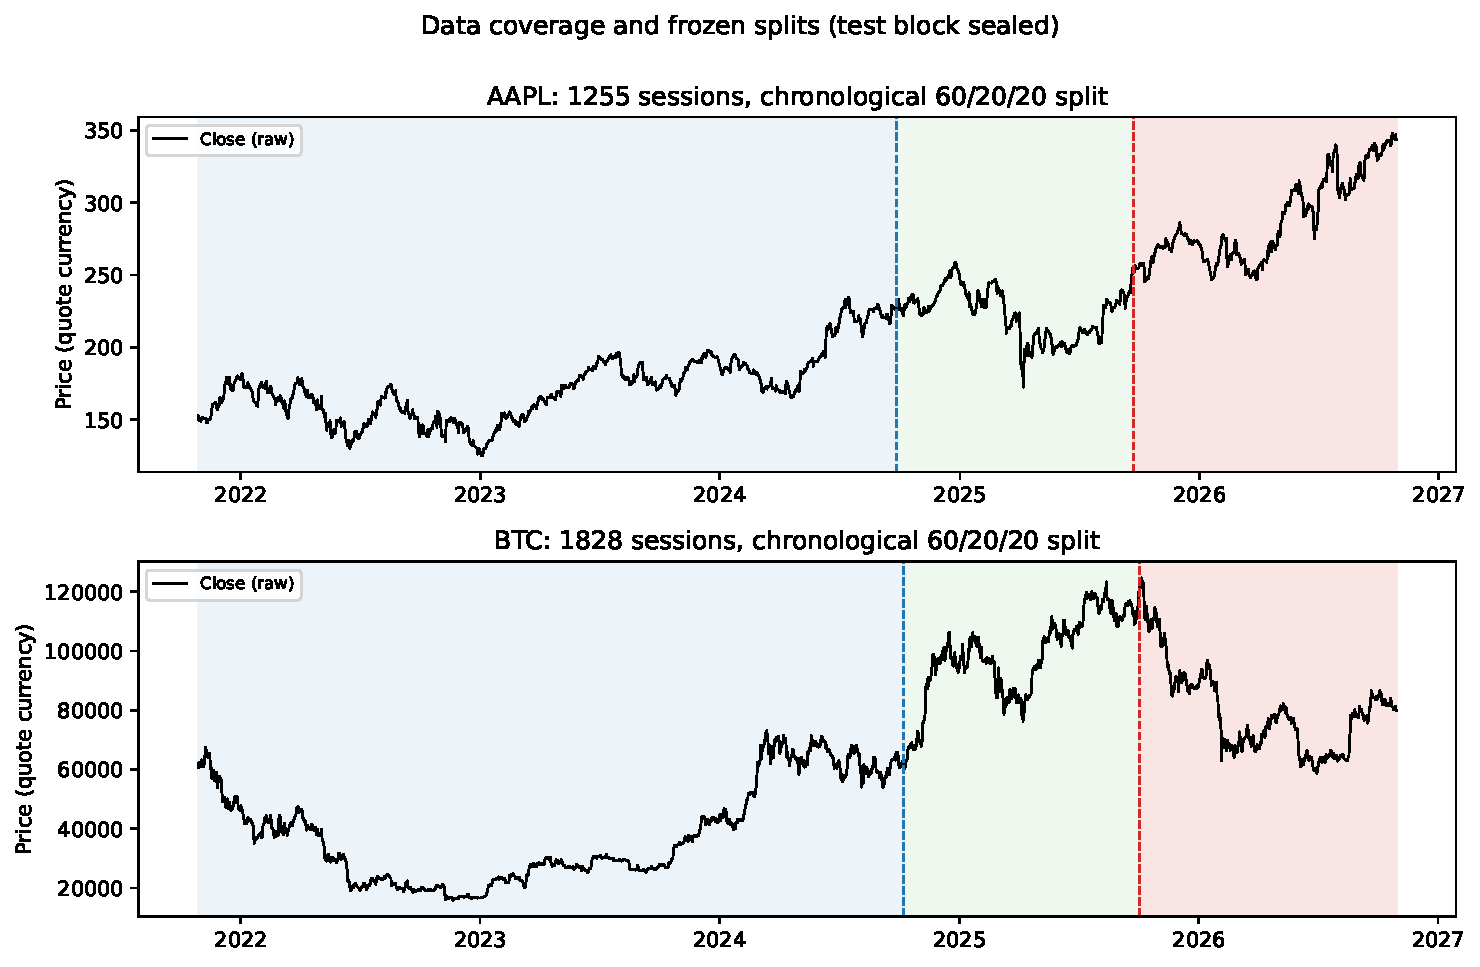
\includegraphics[width=\textwidth,height=0.58\textheight,keepaspectratio]{fig01_coverage_and_splits.pdf}
  \par\vspace{1mm}
  {\footnotesize Blue = training \textperiodcentered{} green = validation
   \textperiodcentered{} \textbf{red = sealed test, never used in these results}}
  \par\vspace{1mm}
  {\scriptsize AAPL validation \ValAAPL{} \textperiodcentered{} BTC validation
   \ValBTC{} \textperiodcentered{} the test block stays closed until the analysis is frozen.}
\end{frame}

\begin{frame}{Ten Signals from the Past}
  \speaker{Dong Yuankun}
  \begin{columns}[T]
    \begin{column}{0.55\textwidth}
      \footnotesize
      Ten trailing quantities, all computable at today's close:
      \begin{itemize}\footnotesize
        \item returns over 1, 5 and 20 sessions
        \item distance from the 5- and 20-session moving average
        \item realised volatility over 10 and 30 sessions
        \item today's high--low range
        \item volume against its recent average
        \item day of the week
      \end{itemize}
    \end{column}
    \begin{column}{0.45\textwidth}
      \begin{block}{All ten are ratios}
        \footnotesize
        None of them is a price. That is deliberate: price levels trend, and a
        model could look good by copying the level.
      \end{block}
      \vspace{1mm}
      \footnotesize
      Cost: the model cannot output a price directly --- which is exactly why
      we predict the change and add it back.
    \end{column}
  \end{columns}
\end{frame}

% ================================================ ACT III — THE REVEAL
% Zhang Yancheng, 6:00 (Acts III and IV, one continuous segment)
\act{Act III: The reveal}

\begin{frame}{What Must Our Models Beat?}
  \speaker{Zhang Yancheng}
  \begin{block}{Naive persistence: tomorrow's close $=$ today's close}
    \footnotesize
    No training, no parameters. For short-horizon prices this is a genuinely
    strong opponent, because daily returns are close to unpredictable.
  \end{block}
  \vspace{1mm}
  \footnotesize
  \begin{columns}[T]
    \begin{column}{0.5\textwidth}
      \textbf{How we score}
      \[
        \text{skill} = 1 - \frac{\text{MAE}_{\text{model}}}{\text{MAE}_{\text{naive}}}
      \]
      \begin{itemize}\footnotesize
        \item $0$ = no better than the simple rule
        \item negative = \emph{worse} than the simple rule
      \end{itemize}
    \end{column}
    \begin{column}{0.5\textwidth}
      \textbf{What the baseline scores}
      \begin{itemize}\footnotesize
        \item AAPL: MAE \$\NaiveMaeAAPL{} over \NValObsAAPL{} sessions
        \item BTC: MAE \NaiveMaeBTC{} over \NValObsBTC{} sessions
      \end{itemize}
      \vspace{1mm}
      {\scriptsize Dollar errors are not comparable between the two assets, so
       comparisons stay within an asset.}
    \end{column}
  \end{columns}
\end{frame}

\begin{frame}{More Complexity, Almost No Improvement}
  \speaker{Zhang Yancheng}
  \centering
  {\scriptsize Standardised variants (P2). Skill in \%; negative means worse
   than persistence. \NRunTotal{} runs in total, \NPairTotal{} asset--model pairs.}
  \vspace{1mm}

  \begin{table}
    \centering\scriptsize
    \setlength{\tabcolsep}{9pt}
    \begin{tabular}{@{}lrrrr@{}}
      \toprule
       & \multicolumn{2}{c}{AAPL} & \multicolumn{2}{c}{BTC} \\
      \cmidrule(lr){2-3}\cmidrule(l){4-5}
      Model & MAE & skill (\%) & MAE & skill (\%) \\
      \midrule
      Linear (near-unreg.) & \MaeAAPLLinearBaseline & \textbf{\SkillAAPLLinearBaseline} & \MaeBTCLinearBaseline & \SkillBTCLinearBaseline \\
      Ridge        & \MaeAAPLRidge & \SkillAAPLRidge & \MaeBTCRidge & \SkillBTCRidge \\
      SVR (RBF)    & \MaeAAPLSvr & \SkillAAPLSvr & \MaeBTCSvr & \SkillBTCSvr \\
      Random forest& \MaeAAPLRandomForest & \textbf{\SkillAAPLRandomForest} & \MaeBTCRandomForest & \SkillBTCRandomForest \\
      Hist.\ boosting & \MaeAAPLHistGradientBoosting & \SkillAAPLHistGradientBoosting & \MaeBTCHistGradientBoosting & \textbf{\SkillBTCHistGradientBoosting} \\
      \midrule
      Naive persistence & \NaiveMaeAAPL & 0.00 & \NaiveMaeBTC & 0.00 \\
      \bottomrule
    \end{tabular}
  \end{table}
  \vspace{1mm}
  {\footnotesize
   Best AAPL: \BestAAPLModelPtwo{} at \BestAAPLSkillPtwo\,\%.
   Best BTC here: \BestBTCModelPtwo{} at \BestBTCSkillPtwo\,\%.
   \NBelowBaseline{} of \NRunTotal{} runs finish \emph{below} the simple rule.}
\end{frame}

\begin{frame}{The Improvements Are Inside the Noise}
  \speaker{Zhang Yancheng}
  \begin{columns}[T]
    \begin{column}{0.56\textwidth}
      \centering
      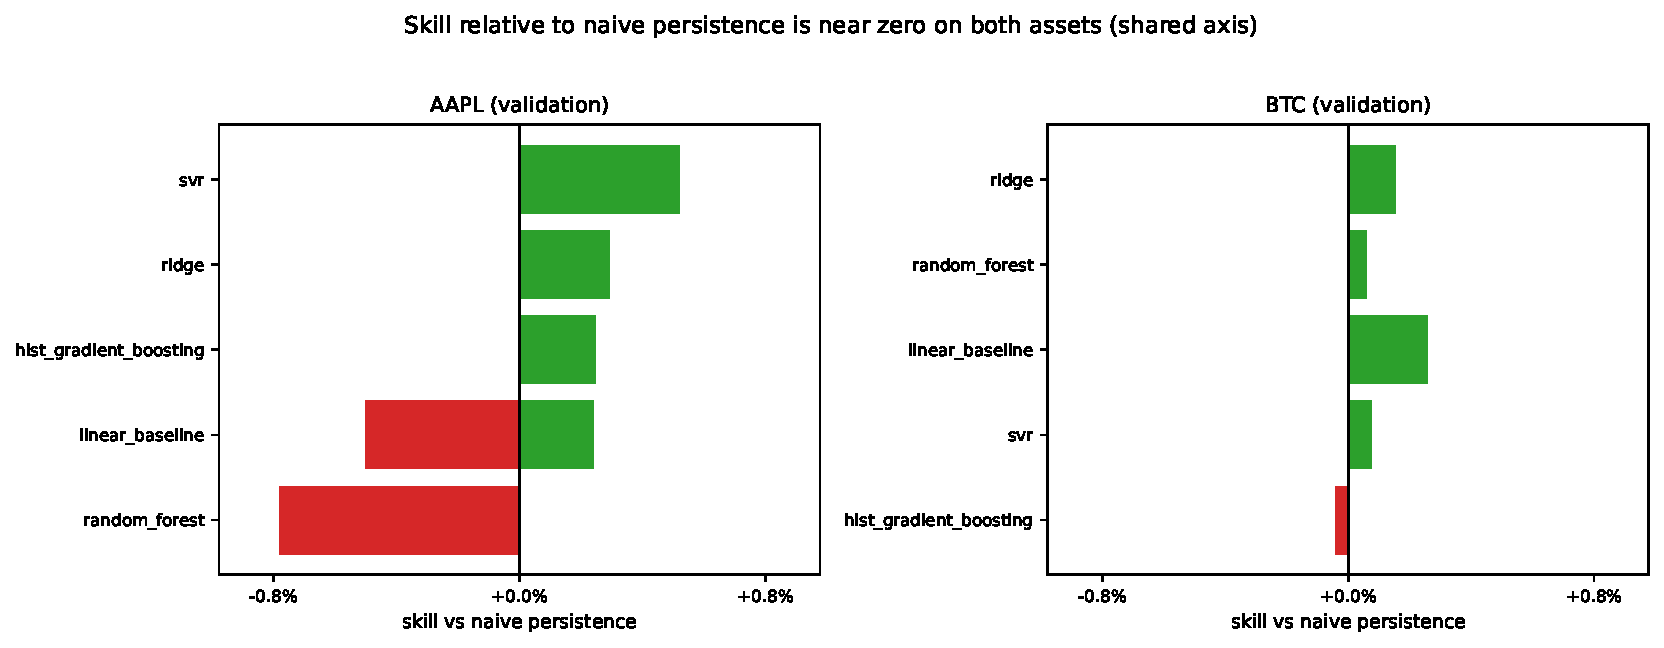
\includegraphics[width=\linewidth]{fig04_model_vs_naive.pdf}
    \end{column}
    \begin{column}{0.44\textwidth}
      \footnotesize
      \begin{itemize}\footnotesize
        \item Every result lies between \SkillMin\% and \SkillMax\% skill ---
              a span of \SkillSpan{} percentage points.
        \item A block-bootstrap interval for skill includes zero for
              \textbf{\NCiIncludeZero{} of \NCiTotal{}} runs.
        \item So we report a \textbf{tie against the baseline}, not a winner.
      \end{itemize}
      \vspace{1mm}
      \begin{alertblock}{Careful wording}
        \footnotesize
        Some configurations are slightly \emph{better} than the rule. None
        establishes a reliable advantage.
      \end{alertblock}
    \end{column}
  \end{columns}
\end{frame}

% =========================================== ACT IV — INVESTIGATING WHY
\act{Act IV: Investigating why}

\begin{frame}{Does Changing the Input Change the Answer?}
  \speaker{Zhang Yancheng}
  \footnotesize
  If more complexity did not help, maybe \emph{how we prepare the data} matters
  more than which model we choose.
  \vspace{1mm}
  \begin{columns}[T]
    \begin{column}{0.47\textwidth}
      \begin{block}{The test}
        \footnotesize
        Same model, same features, same split. The only change: standardise each
        feature (variant P2) instead of leaving it raw (P0).
      \end{block}
      \begin{itemize}\footnotesize
        \item Trees split on \emph{thresholds} in one feature --- rescaling
              preserves order.
        \item Kernel SVR and ridge use \emph{distances and penalties} ---
              rescaling changes the geometry.
      \end{itemize}
    \end{column}
    \begin{column}{0.53\textwidth}
      \centering
      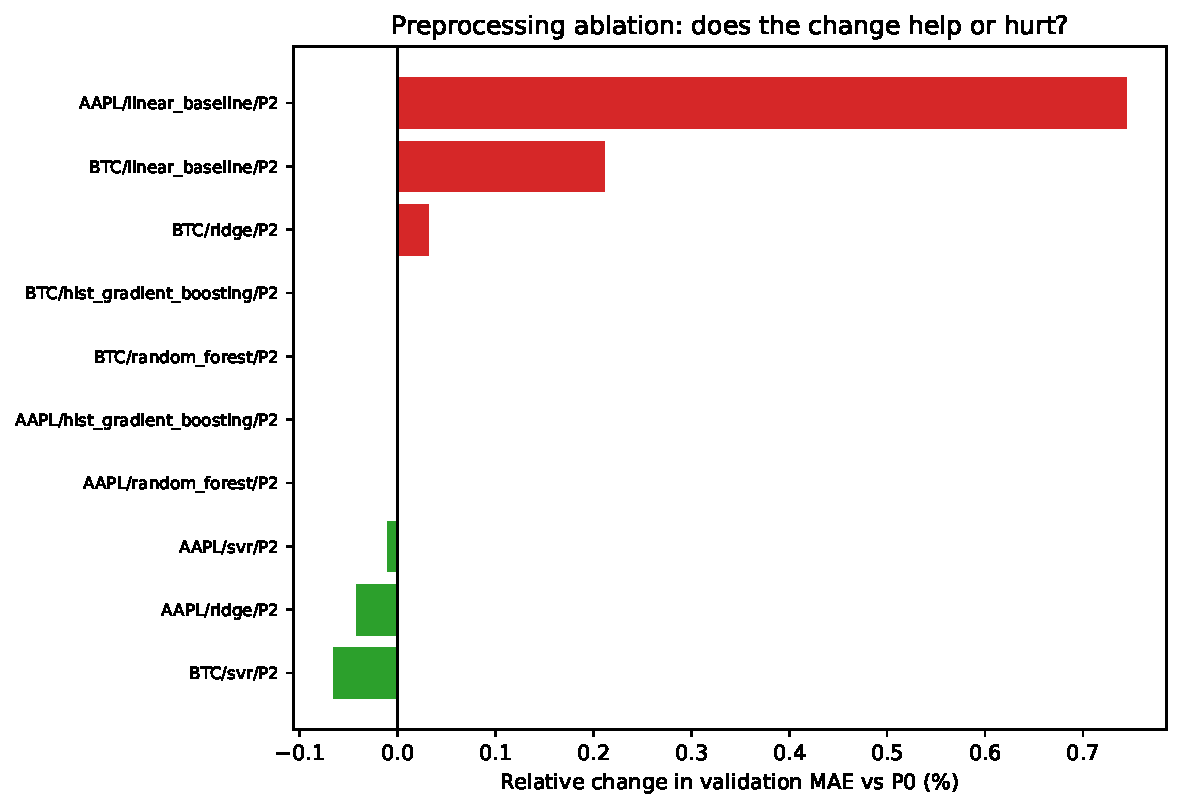
\includegraphics[width=\linewidth,height=0.60\textheight,keepaspectratio]{fig06_ablation_delta.pdf}
    \end{column}
  \end{columns}
  {\footnotesize
   Measured on the committed predictions: for both tree ensembles, scaled and
   unscaled versions differ by \TreeVerdict{} --- identical, as theory predicts.
   Linear and kernel models shift slightly, in both directions.}
\end{frame}

\begin{frame}{Why More Complexity Did Not Help}
  \speaker{Zhang Yancheng}
  \begin{columns}[T]
    \begin{column}{0.52\textwidth}
      \textbf{There is very little short-horizon signal}
      \begin{itemize}\footnotesize
        \item lag-1 autocorrelation of daily returns:
              AAPL \AutoAAPL{}, BTC \AutoBTC{}
        \item that is an $R^2$ of about \AutoRsqAAPL{} and \AutoRsqBTC{}
        \item with little signal, extra capacity fits noise
      \end{itemize}
      \vspace{1mm}
      \textbf{And the tree models have a structural limit}
      \begin{itemize}\footnotesize
        \item a forest predicts an average of training-set leaf values
        \item on a change target that average is small and piecewise constant,
              so it cannot produce large moves
      \end{itemize}
    \end{column}
    \begin{column}{0.48\textwidth}
      \begin{block}{What we did \emph{not} find}
        \footnotesize
        \begin{itemize}\footnotesize
          \item no model family is reliably superior;
          \item preprocessing changes behaviour but does not create edge;
          \item more parameters did not reduce error on unseen dates.
        \end{itemize}
      \end{block}
      \vspace{1mm}
      {\scriptsize This is the honest version of the result, and it is more
       useful than a small, unstable win.}
    \end{column}
  \end{columns}
\end{frame}

% ============================================ ACT V — THE BIGGER LESSON
% Lui Shing Lam, 1:40
\act{Act V: The bigger lesson}

\begin{frame}{What This Teaches Us About Machine Learning}
  \speaker{Lui Shing Lam}
  \begin{enumerate}\small
    \item \textbf{A sophisticated model is not automatically a better model.}
          Five families, including two ensembles, could not clearly beat one line.
    \item \textbf{A fair baseline is not optional.} Without persistence, every
          result here would look like a success.
    \item \textbf{Leakage is easy and invisible.} Our own first test suite missed
          a one-step leak until we tried to break it deliberately.
    \item \textbf{Validation is not the future.} Small differences on one period
          do not survive to new data.
    \item \textbf{Preprocessing depends on the algorithm.} It matters for
          distances, not for thresholds.
  \end{enumerate}
  \vspace{1mm}
  {\footnotesize The project also ships a lesson with five worked exercises and a
   notebook that re-runs the comparison. It is a \emph{designed} resource --- we
   ran no learner study, so we claim no measured learning gain.}
\end{frame}

\begin{frame}{The Value Is in the Comparison}
  \speaker{Lui Shing Lam}
  \begin{columns}[T]
    \begin{column}{0.5\textwidth}
      \textbf{Limits, stated plainly}
      \begin{itemize}\footnotesize
        \item two assets, one period, one-day horizon
        \item BTC is one venue's USDT price
        \item one-day forecasting is where the simple rule is strongest
        \item our test block is still sealed --- these are validation results
      \end{itemize}
    \end{column}
    \begin{column}{0.5\textwidth}
      \begin{block}{The takeaway}
        \small
        The value of machine learning is not measured by how complicated a model
        is, but by whether it learns something useful beyond a meaningful
        baseline.
      \end{block}
      \vspace{2mm}
      \begin{alertblock}{}
        \footnotesize Historical, educational analysis --- \textbf{not investment
        advice}. Forecast error does not imply profit.
      \end{alertblock}
    \end{column}
  \end{columns}
\end{frame}

% ==================================================================== BACKUP
% \appendix makes beamer write \translate into the PDF bookmark string, which
% hyperref strips with a warning. Setting the bookmark text directly avoids it.
\appendix
\section{Backup material}
\setbeamertemplate{footline}{\intfootline}

\begin{frame}{Backup: Every Configuration, Not Just the Ones We Showed}
  \speaker{Zhang Yancheng}
  \centering
  {\scriptsize Skill (\%) for every model, asset and variant --- evidence that the
   P2 table was not cherry-picked.\par}
  \vspace{1mm}
  % A bare \input of a tabular would be typeset inline inside the paragraph
  % above and overlap it; the center environment forces its own paragraph.
  \begin{center}
    \scriptsize
    \setlength{\tabcolsep}{7pt}
    % GENERATED by scripts/build_slide_assets.py -- do not edit by hand.
% Backup slide: skill (\%) for every model, asset and preprocessing variant.
\begin{tabular}{@{}lrrrr@{}}
\toprule
 & \multicolumn{2}{c}{AAPL} & \multicolumn{2}{c}{BTC} \\
\cmidrule(lr){2-3}\cmidrule(l){4-5}
Model & P0 & P2 & P0 & P2 \\
\midrule
Linear (near-unregularised) & +0.24 & -0.50 & +0.26 & +0.05 \\
Ridge & +0.25 & +0.29 & +0.15 & +0.12 \\
SVR (RBF) & +0.51 & +0.52 & +0.01 & +0.08 \\
Random forest & -0.78 & -0.78 & +0.06 & +0.06 \\
Hist.\ gradient boosting & +0.25 & +0.25 & -0.04 & -0.04 \\
\midrule
Naive persistence & 0.00 & 0.00 & 0.00 & 0.00 \\
\bottomrule
\end{tabular}

  \end{center}
  {\scriptsize Best BTC overall is \BestBTCModelAll{} (\BestBTCVariantAll{}) at
   \BestBTCSkillAll\,\%, just above the best P2 value. Validation statistics only;
   \NCiIncludeZero{}/\NCiTotal{} bootstrap intervals include zero.\par}
\end{frame}

\begin{frame}{Backup: Was the Comparison Fair?}
  \speaker{Zhang Yancheng}
  \begin{itemize}\footnotesize
    \item Identical features, split, target and evaluation dates for every
          model.
    \item Identical search budget: \TrialsUsed{} random trials, at most
          \SecondsUsed{} seconds per cell (\BudgetUniform{} across all
          \NRunTotal{} runs).
    \item The frozen protocol allows up to \TrialsMax{} trials / \SecondsMax{}s;
          the committed runs used the reduced budget, and we report the budget
          that was actually used.
    \item Tuning ran only inside the training block, so validation stayed a
          selection holdout.
    \item Every estimator is built through one code path, so no lane silently
          receives different columns.
  \end{itemize}
\end{frame}

\begin{frame}{Backup: How We Caught Our Own Leak}
  \speaker{Dong Yuankun}
  \begin{itemize}\footnotesize
    \item An independent audit found that the last training label was a
          validation price, and the last validation label a \emph{sealed test}
          price. Perturbing one test price moved the reported metric by
          \textbf{0.408} --- far more than any model's advantage.
    \item Fix: purge one row at each boundary. A protocol check now refuses a
          purge smaller than the forecast horizon.
    \item The audit also showed our leakage tests could not detect a one-step
          forward shift. We added independent-formula checks and a mutation
          harness: six known defects, six caught.
    \item A second audit, run in a separate context, re-derived the boundaries
          and wrote its own obfuscated defects. Both were caught.
  \end{itemize}
\end{frame}

\begin{frame}{Backup: What the Fitted Model Relies On}
  \speaker{Zhang Yancheng}
  \begin{columns}[T]
    \begin{column}{0.55\textwidth}
      \centering
      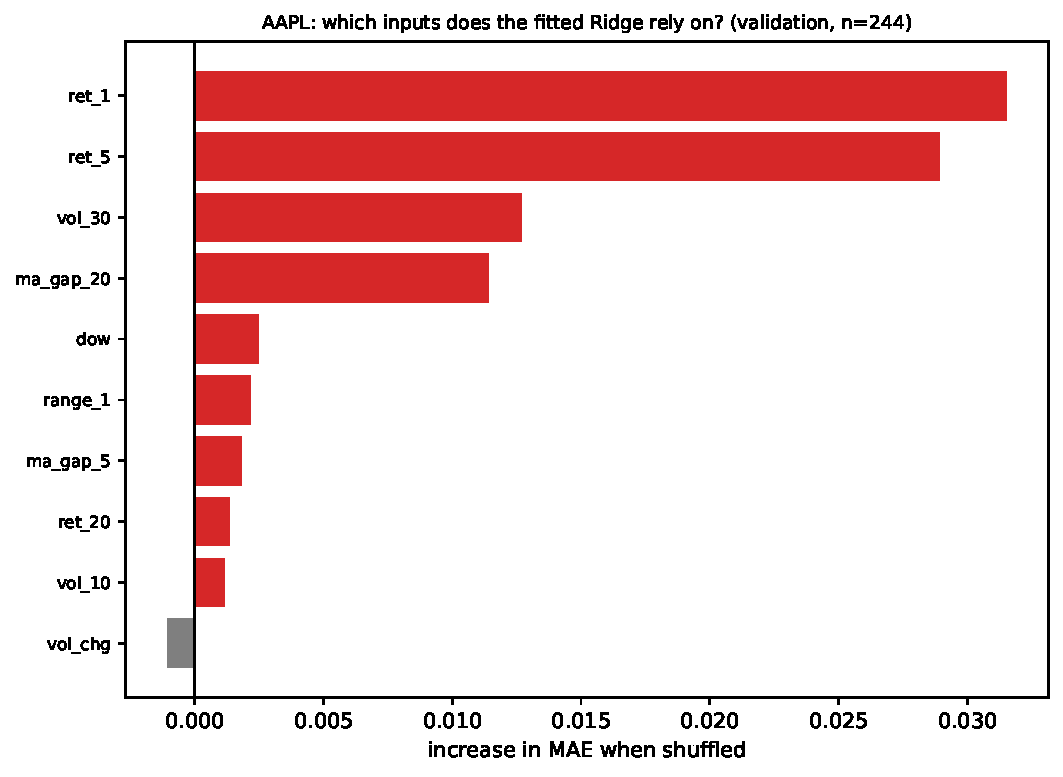
\includegraphics[width=\linewidth]{fig07_feature_importance_aapl.pdf}
    \end{column}
    \begin{column}{0.45\textwidth}
      \footnotesize
      Permutation importance: shuffle one feature, measure the increase in
      validation error, for the ridge model on AAPL.
      \vspace{1mm}
      \begin{itemize}\footnotesize
        \item short-horizon returns and volatility dominate
        \item the magnitudes are tiny --- consistent with the skill table
        \item this describes the fitted model, not a cause in the market
      \end{itemize}
    \end{column}
  \end{columns}
\end{frame}

\begin{frame}{Backup: Questions and Who Answers Them}
  \speaker{All five presenters}
  \begin{table}\footnotesize
    \setlength{\tabcolsep}{4pt}
    \begin{tabular}{@{}p{0.5\textwidth}p{0.42\textwidth}@{}}
      \toprule
      Question & Presenter \\
      \midrule
      Isn't this just a random walk? & Zhang Yancheng \\
      Did you leak future data? & Dong Yuankun \\
      Why no LSTM or deep learning? & Zhang Yancheng \\
      Is a 0.5\% improvement meaningful? & Zhang Yancheng \\
      Why does BTC need a different model? & Zhang Haoyu \\
      What should students learn from this? & Lui Shing Lam \\
      Can this be used for trading? & Lau Pak Hei \\
      \bottomrule
    \end{tabular}
  \end{table}
  \vspace{1mm}
  {\scriptsize Speaking roles are presentation roles only. Research and software
   ownership is recorded separately in \texttt{docs/management/responsibilities.md}.}
\end{frame}

\end{document}
